\subsection{Strategi \textit{Deployment} \textsc{Nginx}}

\begin{enumerate}
	\item CORS (\textit{Cross Origin Resource Sharing})
	\\
	CORS adalah sebuah mekanisme yang memungkinkan  sebuah \textit{website} menggunakan \textit{resources}(seperti skrip Javascript, \textit{fonts}, dll) untuk diakses dari sumber lain selain \textit{domain origin}nya.Secara teknis, CORS mendefinisikan \textit{protokol}/cara browser dan server untuk berinteraksi otorisasi permintaan \textit{resource} dari domain lain, dan juga lebih aman karena \textit{developer} dapat mengkontrol otorisasi tersebut (daripada mengizinkan semua permintaan).\\
	
	% todo cite wikipedia
	\textbf{\textit{The Problem}} \\
	Masalah koneksi ke server lelang (yang berjalan pada domain yang sama, namun port yang berbeda) tidak dapat tersambung karena \textit{error} berikut :


	\begin{figure}[H]
		\centering
		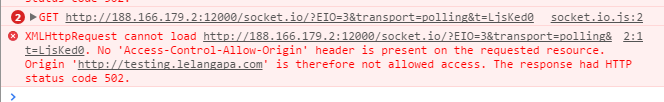
\includegraphics[width=\textwidth]{images/bab4/pl/madafaka_cors.png}
		\caption{\textit{Error} CORS yang muncul pada console browser}
		\label{cors}
	\end{figure}
	
	
	\textbf{\textit{Insight}} \\
	Selama 2 minggu kurang lebih penulis mencoba cara yang ditemukan penulis dalam situs stackoverflow untuk mengkonfigurasi \textit{server} lelang agar otorisasi CORS dapat dilakukan, namun tidak ada hasil.\\
	\indent Masalah ini terselesaikan setelah menggunakan fitur \textit{reverse proxy} dari Nginx.\\
	
	\textbf{\textit{Solution}} \\
	\indentenum Strateginya adalah sebagai berikut :
	\begin{enumerate}
		\item \label{nginx-a} \textit{Server} lelang berjalan pada localhost port 3000.
		\item \label{nginx-b} Diatur sebuah subdomain khusus -- misalkan A.domain.com
		\item \textsc{Nginx} dikonfigurasi dimana semua \textit{requests} menuju A.domain.com ke aplikasi \textit{localhost} yang kita maksud di poin \ref{nginx-a}
		\item Selain meneruskan \textit{requests}, \textsc{Nginx} juga akan meneruskan \textit{reply} dari server lelang tersebut kepada \textit{client}/\textit{origin} yang meminta \textit{request} tersebut.				
	\end{enumerate}
\end{enumerate}